\documentclass{article}
\usepackage[utf8]{inputenc}
\usepackage{graphicx}
\usepackage{wrapfig}
\usepackage{array}
\usepackage{siunitx}
\usepackage{xcolor}
\usepackage{multicol}
\usepackage{amssymb}
\usepackage{hyperref}
\setlength{\columnseprule}{1pt}

\title{Applications of Diode \\ Lab Report 5 \\ ELP100}
\author{Yash Agarwal \\ 2021EE10638 \\ Group 29}
\date{May 21, 2022}

\begin{document}
\pagecolor{yellow!15}
\maketitle
\vspace{15px}
\tableofcontents
\newcolumntype{V}{>{\centering\arraybackslash} m{.4\linewidth} }
\newpage
\section{Half Wave Rectifier}
\subsection{Aim}
To investigate the characteristic of diode half wave rectifier.
\subsection{Apparatus}
\begin{enumerate}
\item Breadboard and Jumpers
\item Multimeter and Resistors
\item Capacitor ( Both Electrolytic and Non-Electrolytic)
\item Digital Storage Oscilloscope (DSO1052B)
\item Function Generator (0 – 3 MHz)
\end{enumerate}

\subsection{Theory}
\begin{wrapfigure}{R}{0.35\textwidth}
\fcolorbox{black}{white}{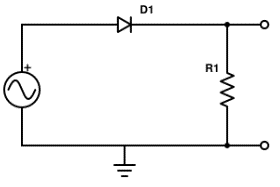
\includegraphics[width=0.35\textwidth]{Picture1.png}}
\end{wrapfigure}
The diode when forward biased will allow current to flow, i.e., in the positive half cycle of the ac source, it will behave normally like a short or a small resistance. But when reverse biased, the diode will not allow any flow of current, posing as an almost infinitely large resistance. \\


\noindent
Diode half wave rectifier:
\begin{itemize}
\item Rectification is a process of conversion from AC to DC.
\item During +ve half cycle: – Diode is forward biased – Conducts current through RL
\item During -ve half cycle: – Diode is reverse biased – No current flow through the circuit
\item Only +ve half cycle appears across the load ($R_L$), whereas, the –ve half cycle is suppressed
\end{itemize}

\newpage

\subsection{Breadboard Setup}
\vspace{5px}
\begin{multicols}{2}
\begin{center}
\fcolorbox{black}{white}{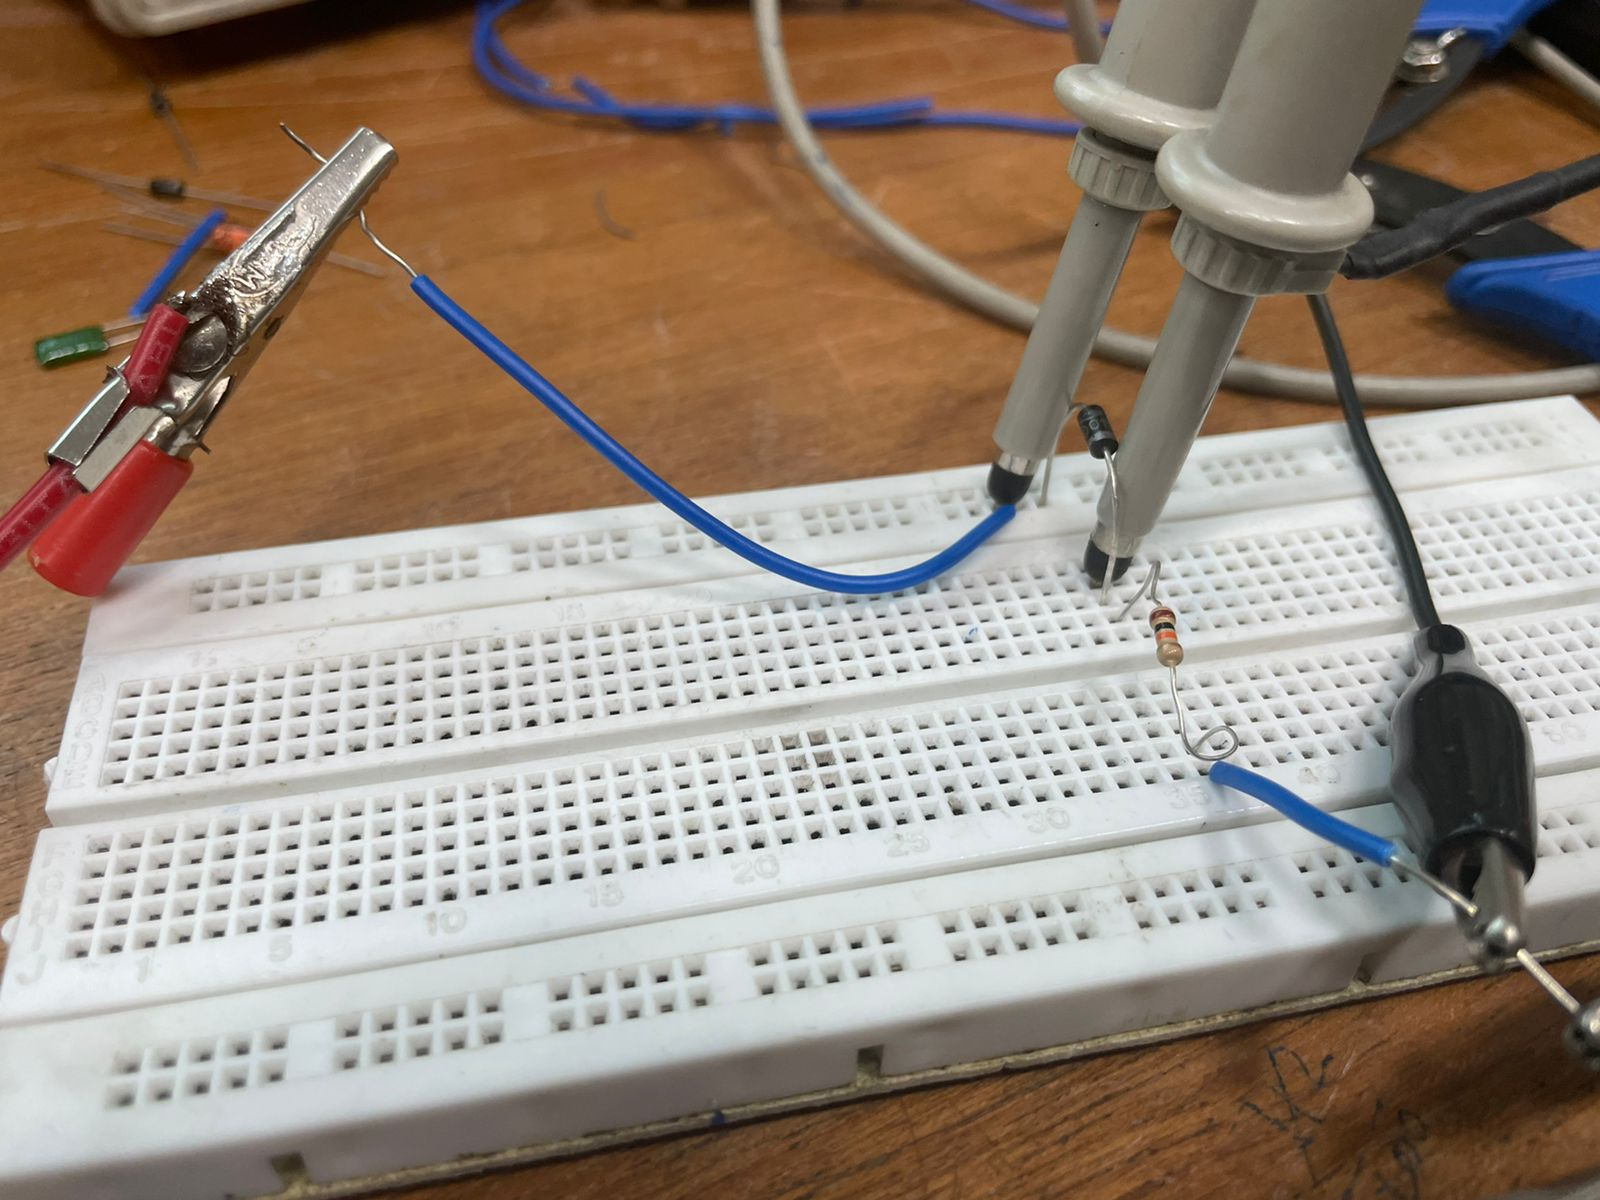
\includegraphics[width=0.9\columnwidth, height=110px]{withoutcap.jpeg}} \\ \vspace{5px}
Circuit with $R=10k\Omega$\\

\columnbreak

\fcolorbox{black}{white}{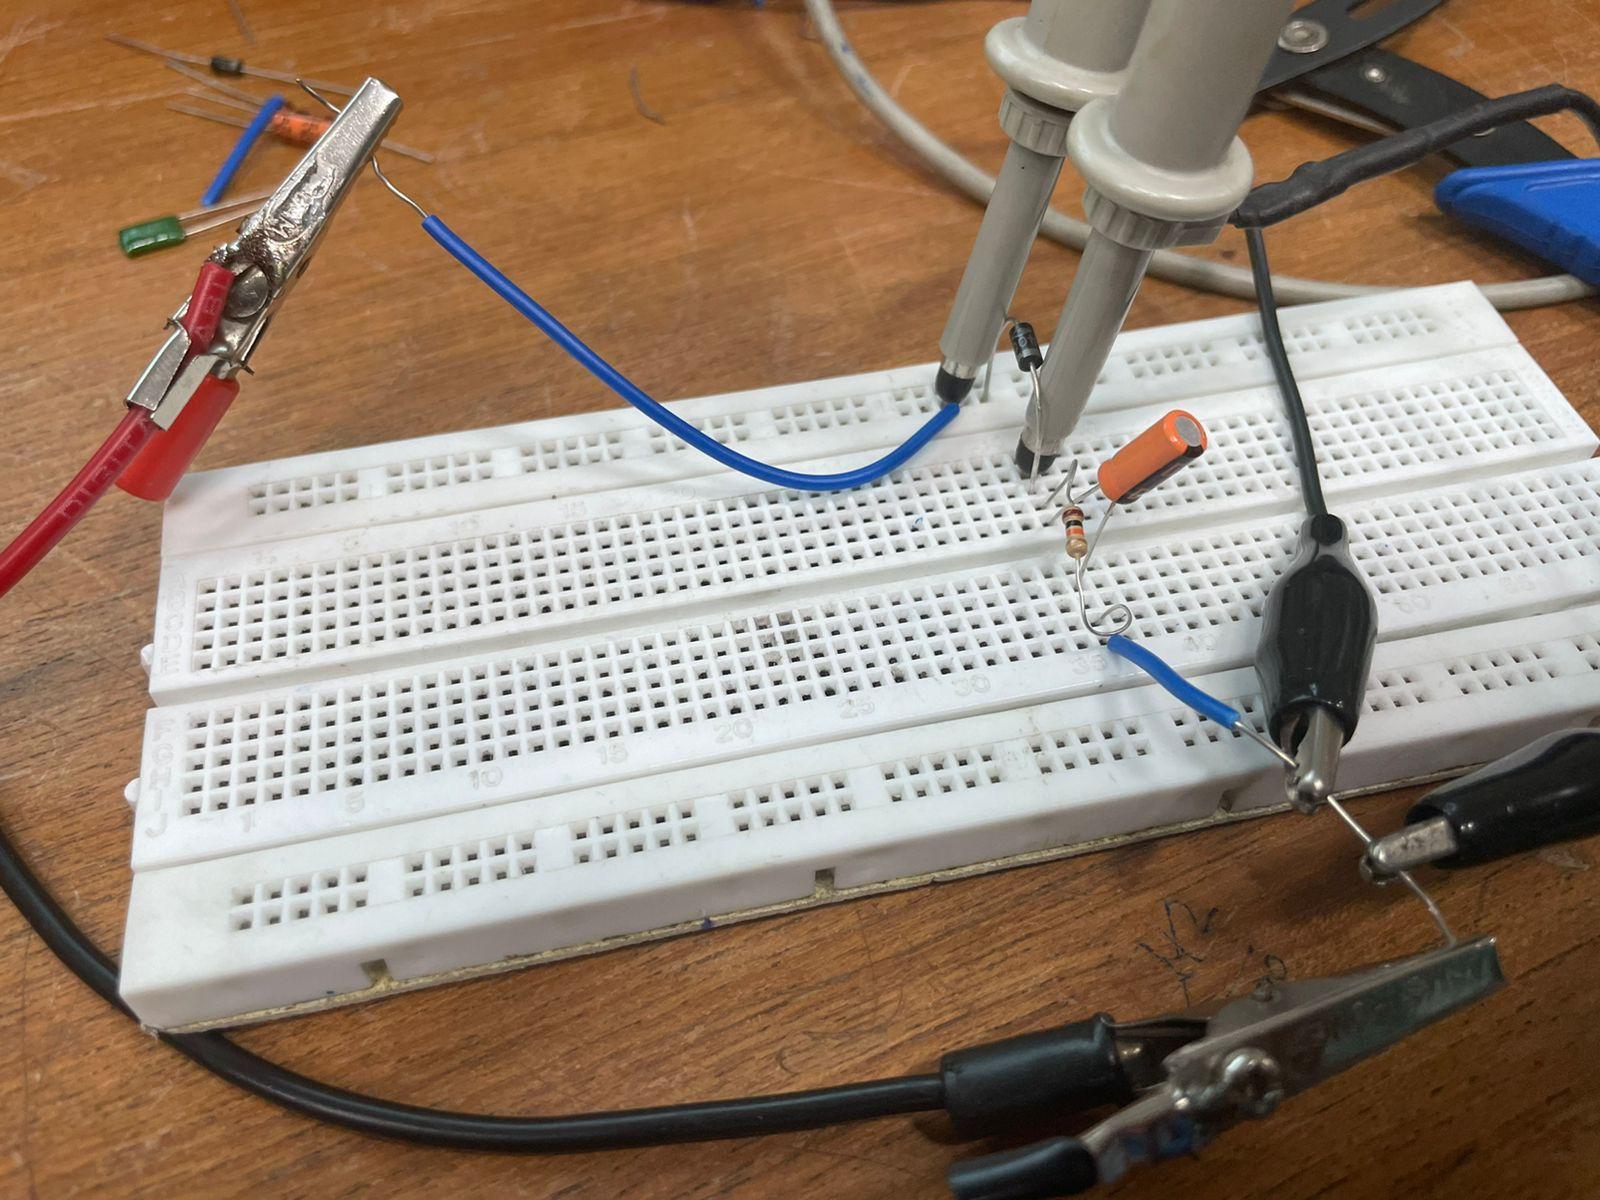
\includegraphics[width=0.9\columnwidth, height=110px]{withcap.jpeg}} \\ \vspace{5px}
Circuit with Electrolytic Capacitor in Parallel
\end{center}
\end{multicols}

\subsection{Images of DSO}
\vspace{5px}
\begin{multicols}{2}
\begin{center}
\fcolorbox{black}{white}{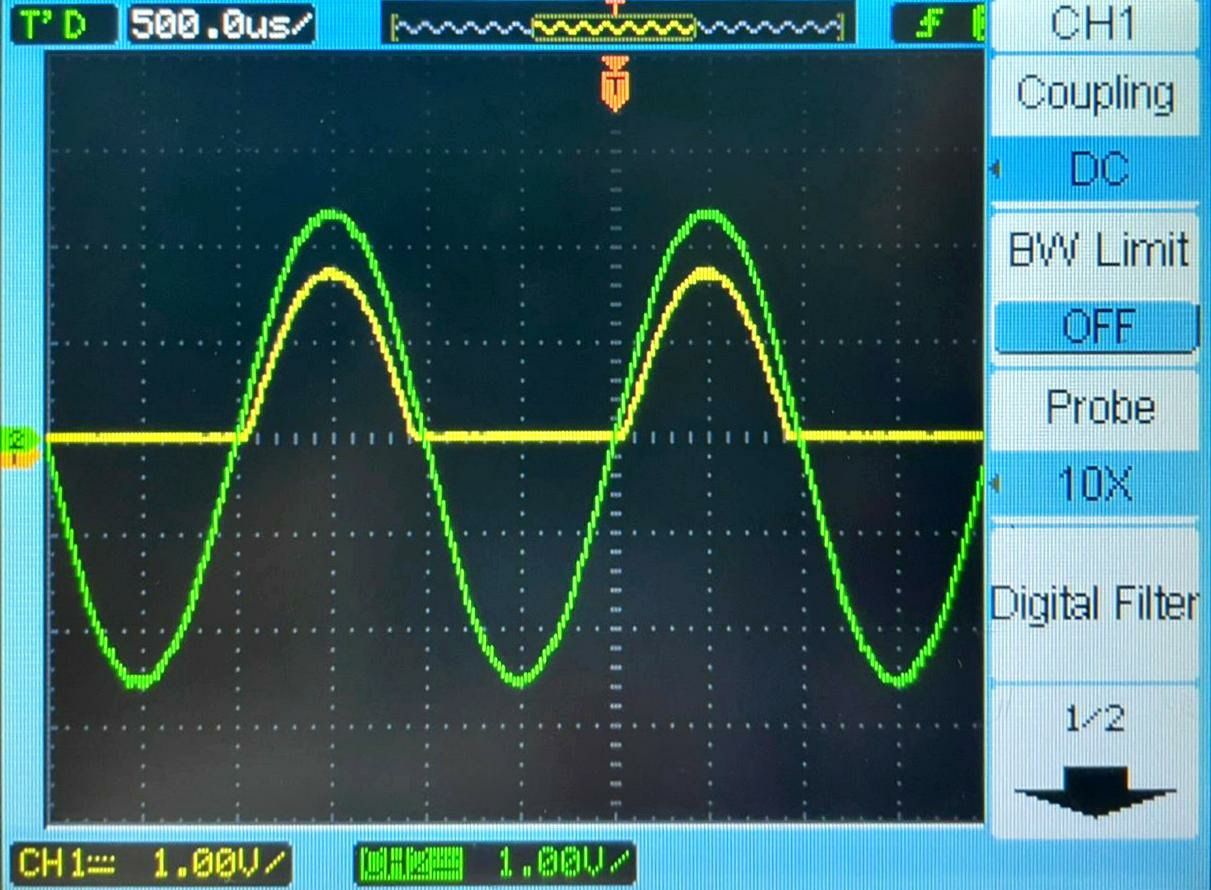
\includegraphics[width=0.9\columnwidth, height=110px]{r.jpeg}} \\ \vspace{5px}
Voltage with Resistor\\

\columnbreak

\fcolorbox{black}{white}{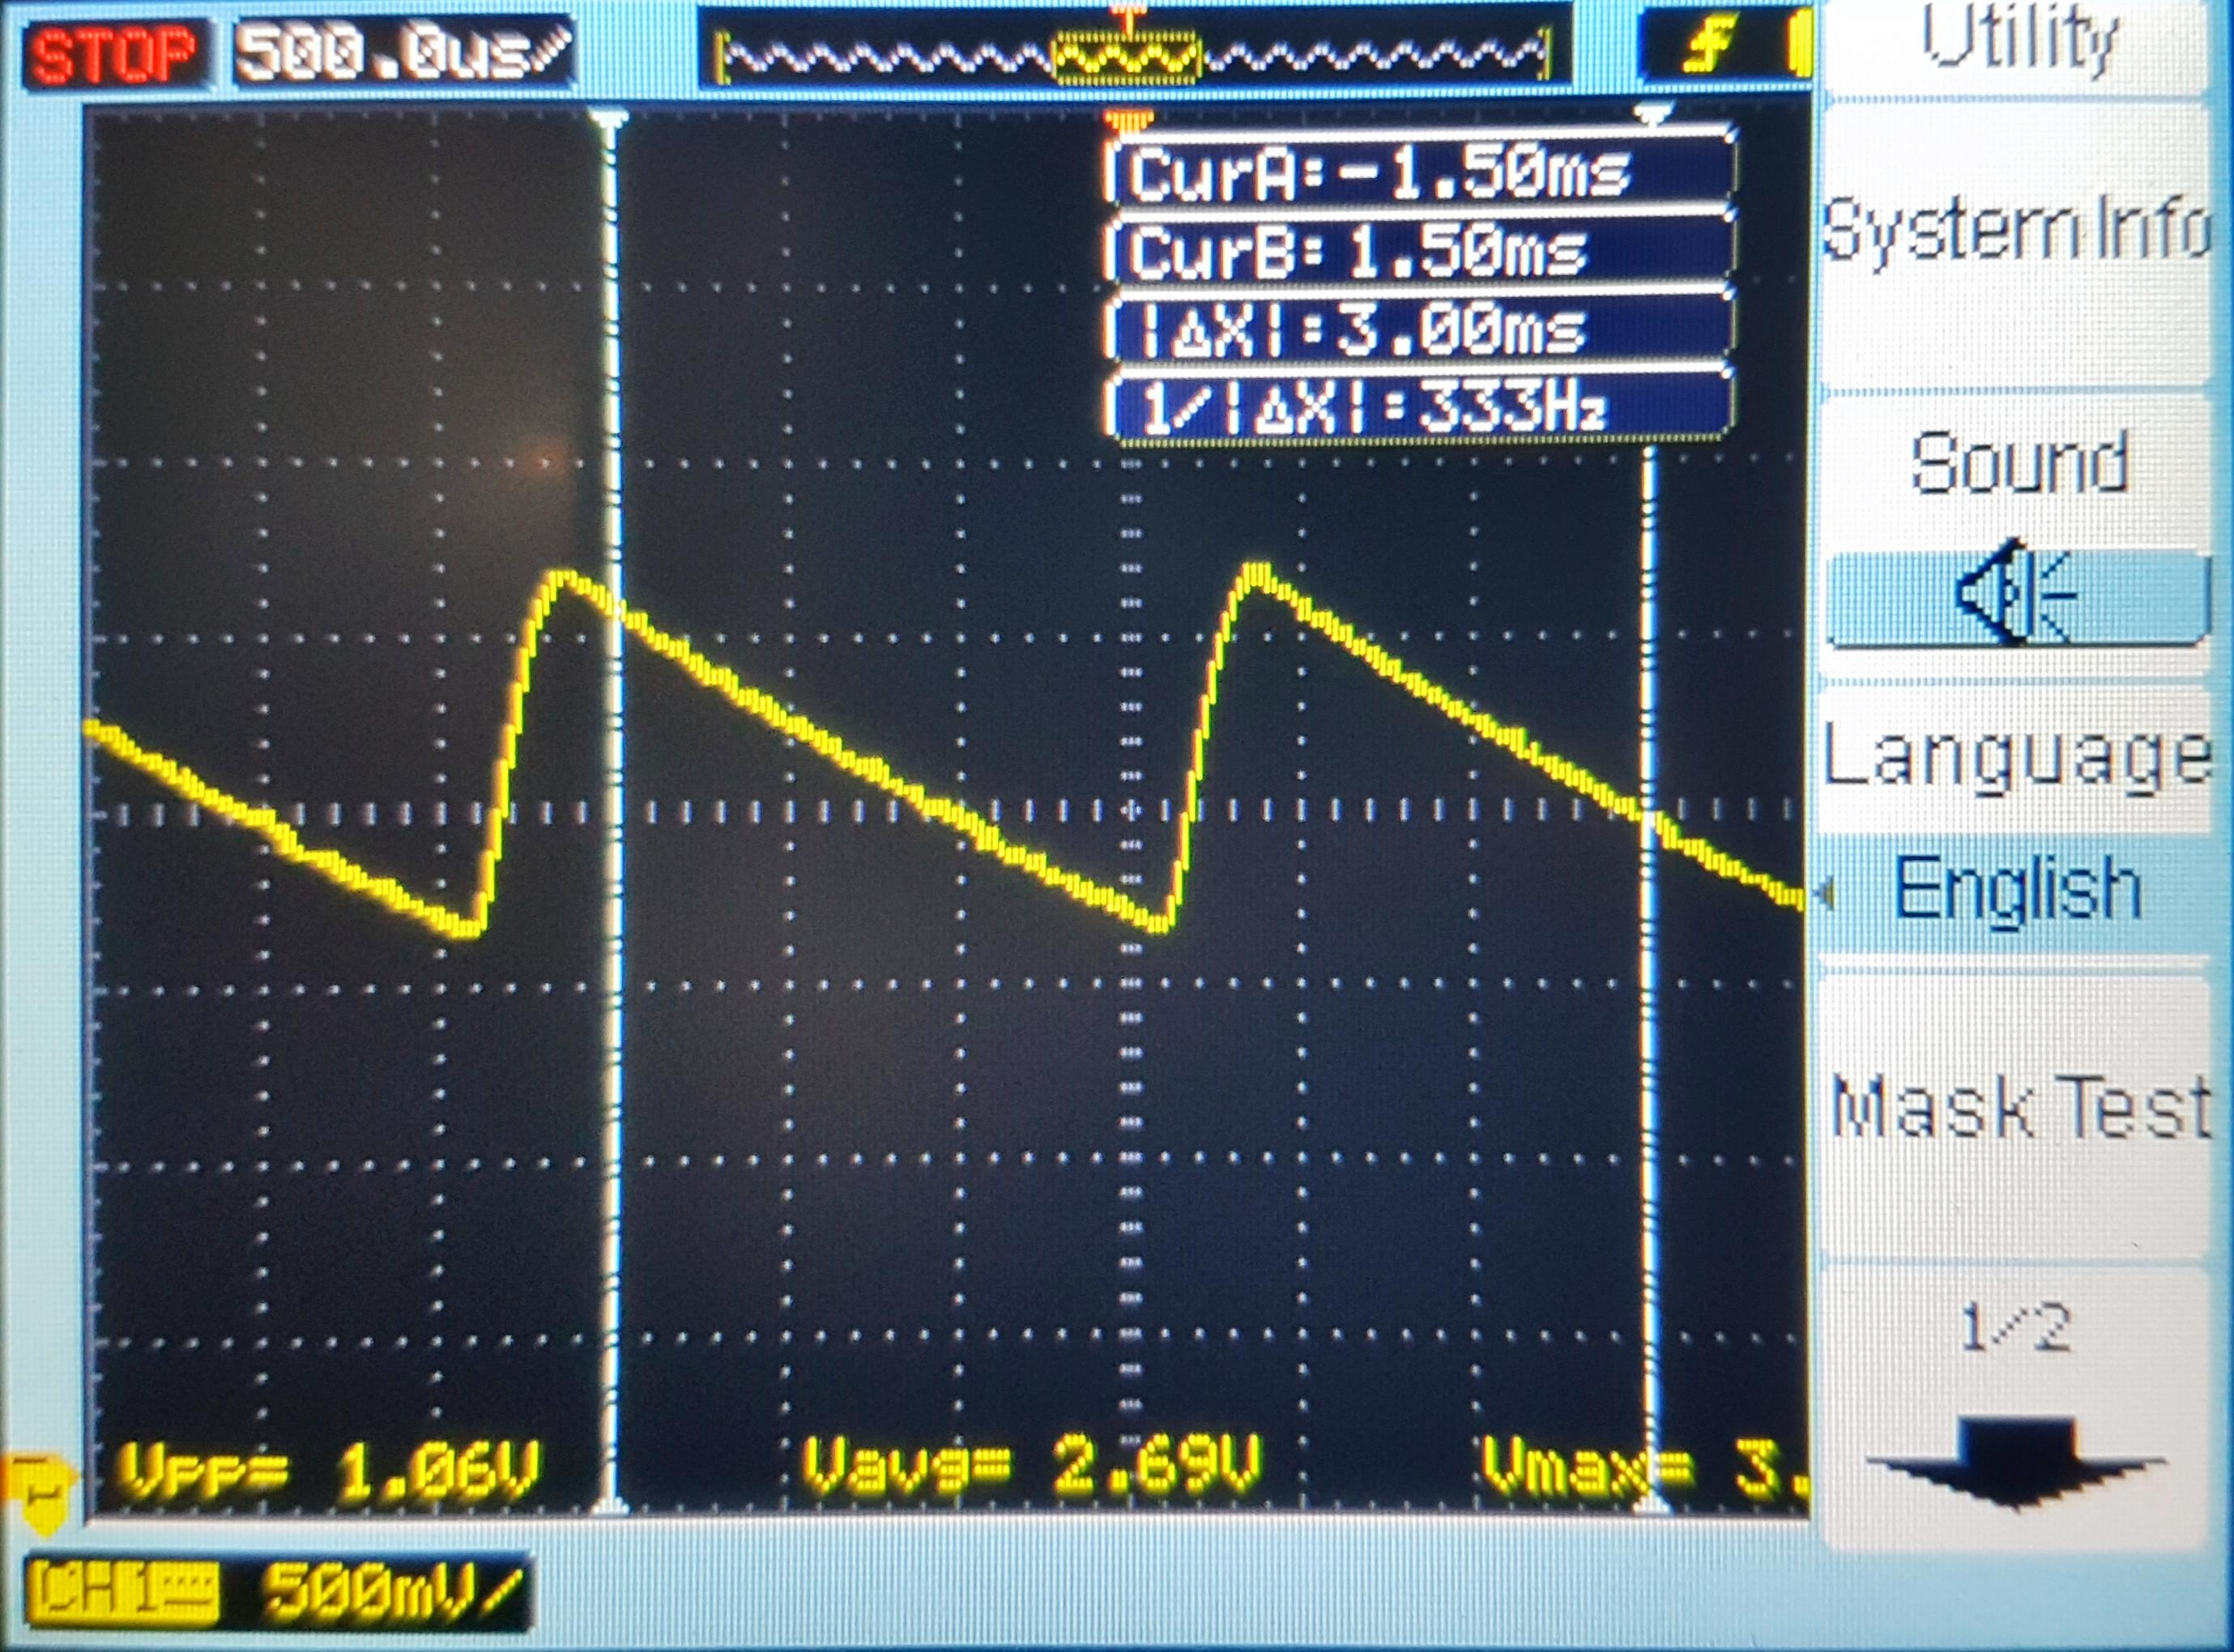
\includegraphics[width=0.9\columnwidth, height=110px]{c.jpeg}} \\ \vspace{5px}
Voltage with Resistor and Capacitor
\end{center}
\end{multicols}

\subsection{Observation}
\vspace{5px}
\begin{center}
\begin{tabular}{| c | c | c | c |} 
 \hline
    \ & \ & \ & \ \\
    $V_0=5V$ &$V_{Input}$ & $V_{Output}$ & $V_{Output}$ with Capacitor \\ [1em]
    \hline
    \ & \ & \ & \ \\
    $V_{PP}$ & 4.88V & 1.76V & 0.53V \\
    $V_{avg}$ & -58.3mV & 517mV & 1.34V \\
    \ & \ & \ & \ \\
 \hline
\end{tabular}
\end{center}
\vspace{5px}
\begin{center}
\begin{tabular}{| c | c | c | c |} 
 \hline
    \ & \ & \ & \ \\
    $V_0=0.5V$ &$V_{Input}$ & $V_{Output}$ & $V_{Output}$ with Capacitor \\ [1em]
    \hline
    \ & \ & \ & \ \\
    $V_{PP}$ & 480mV & 126mV & 23mV \\
    $V_{avg}$ & -9.87mV & 49.93mV & 37mV \\
    \ & \ & \ & \ \\
 \hline
\end{tabular}
\end{center}

\subsection{Conclusion}
Hence we see the ouput waveforms for a Half-wave Rectifier in the case of a simple resistor and when capacitor smoothing happens.

\vspace{20px}
\section{Diode Clipping}
\subsection{Aim}
To investigate the characteristic of diode clipping circuit.
\subsection{Apparatus}
\begin{enumerate}
\item Breadboard and Jumpers
\item Multimeter and Resistors
\item Capacitor ( Both Electrolytic and Non-Electrolytic)
\item Digital Storage Oscilloscope (DSO1052B)
\item Function Generator (0 – 3 MHz) and External Voltage
\end{enumerate}

\subsection{Theory}
\begin{wrapfigure}{R}{0.25\textwidth}
\fcolorbox{black}{white}{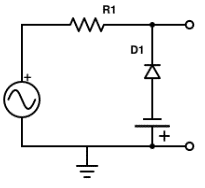
\includegraphics[width=0.25\textwidth]{Picture2.png}}
\end{wrapfigure}
Simple diode clipper can be made with a diode and a resistor. The simple circuit clips at zero voltage (or to be more precise, at the small forward voltage of the forward biased diode) but the clipping voltage can be set to any desired value with the addition of a reference voltage. The diagram illustrates a negative reference voltage but the reference can be positive or negative for both positive and negative clipping giving four possible configurations in all. The diode polarity decides the half cycle which will be affected, i.e, where the clipping will take place, and the source voltage decides the magnitude at which he signal is to be clipped. \\

\noindent
\textbf{Diode and Source Polarities are considered +ve as per the circuit on the right.}

\subsection{Breadboard Setup}
\vspace{5px}
\begin{center}
\fcolorbox{black}{white}{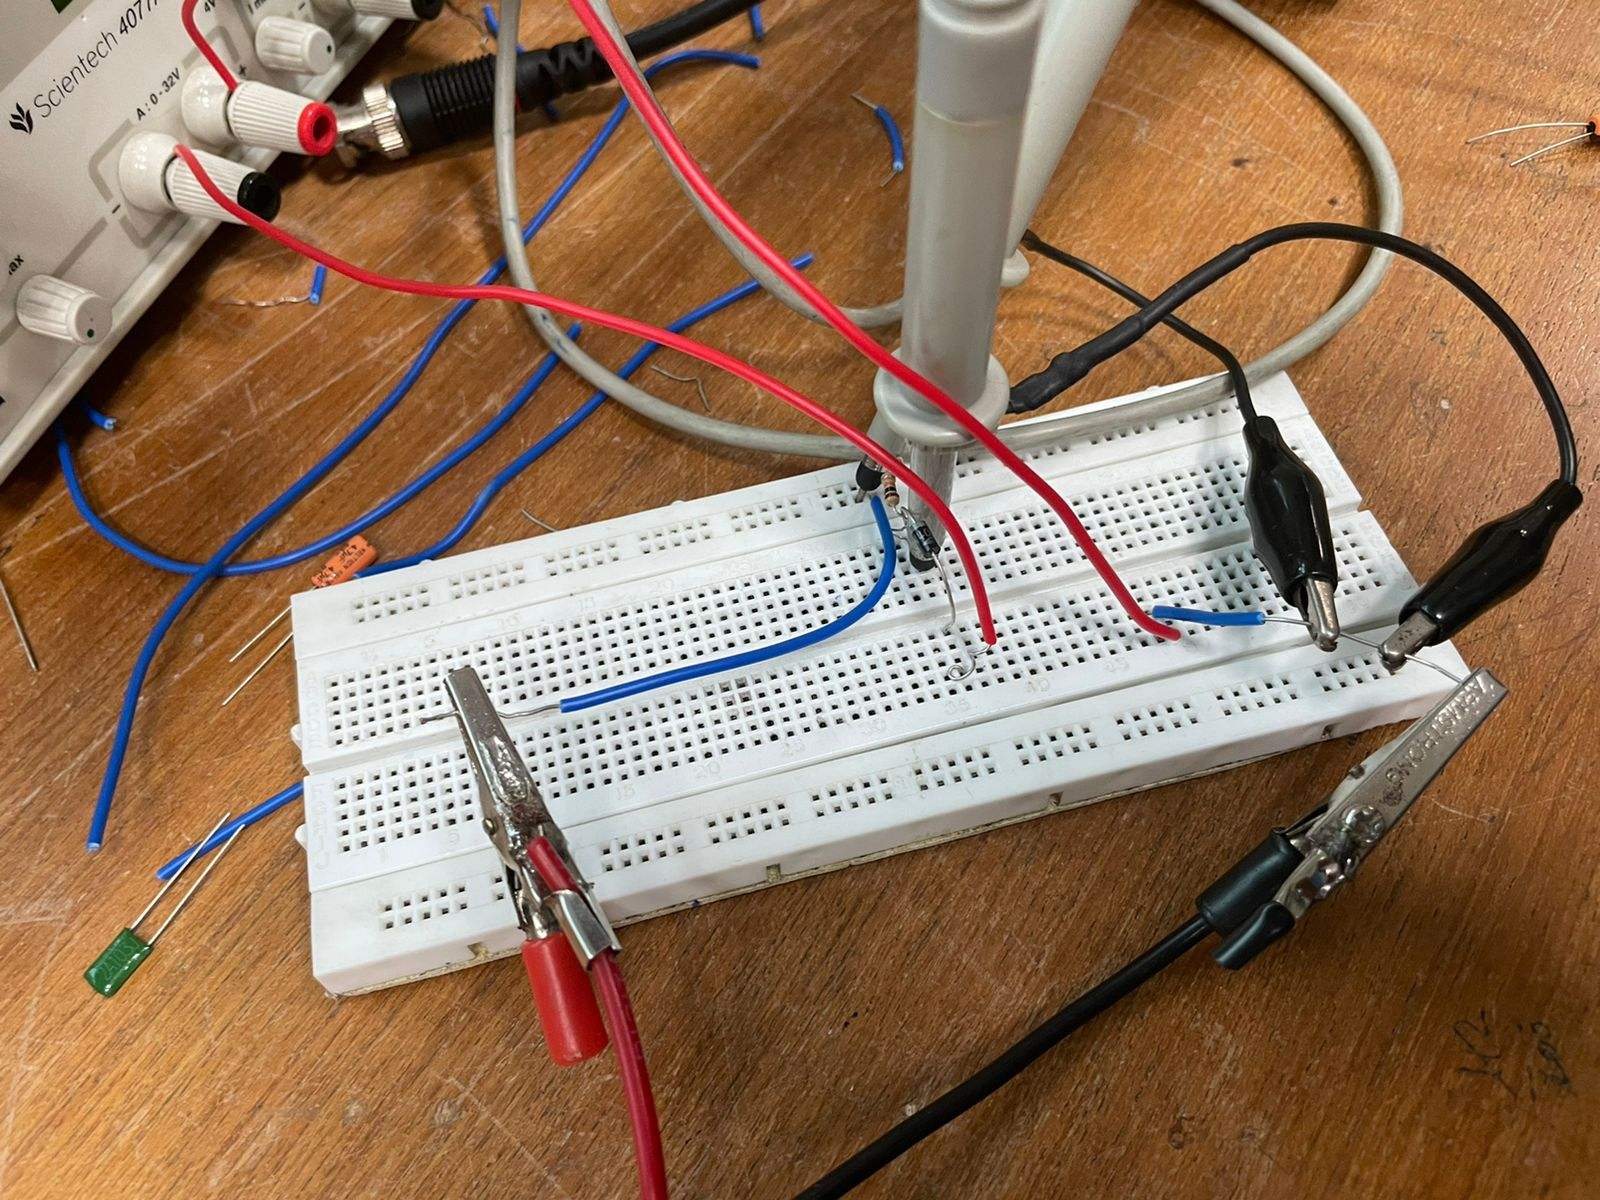
\includegraphics[width=0.9\columnwidth, height=150px]{WhatsApp Image 2022-04-27 at 4.39.46 PM.jpeg}} \\ \vspace{5px}
Circuit with $R=10k\Omega$ and V=2V\\
\end{center}


\subsection{Images of DSO}
\vspace{5px}
\begin{multicols}{2}
\begin{center}
\fcolorbox{black}{white}{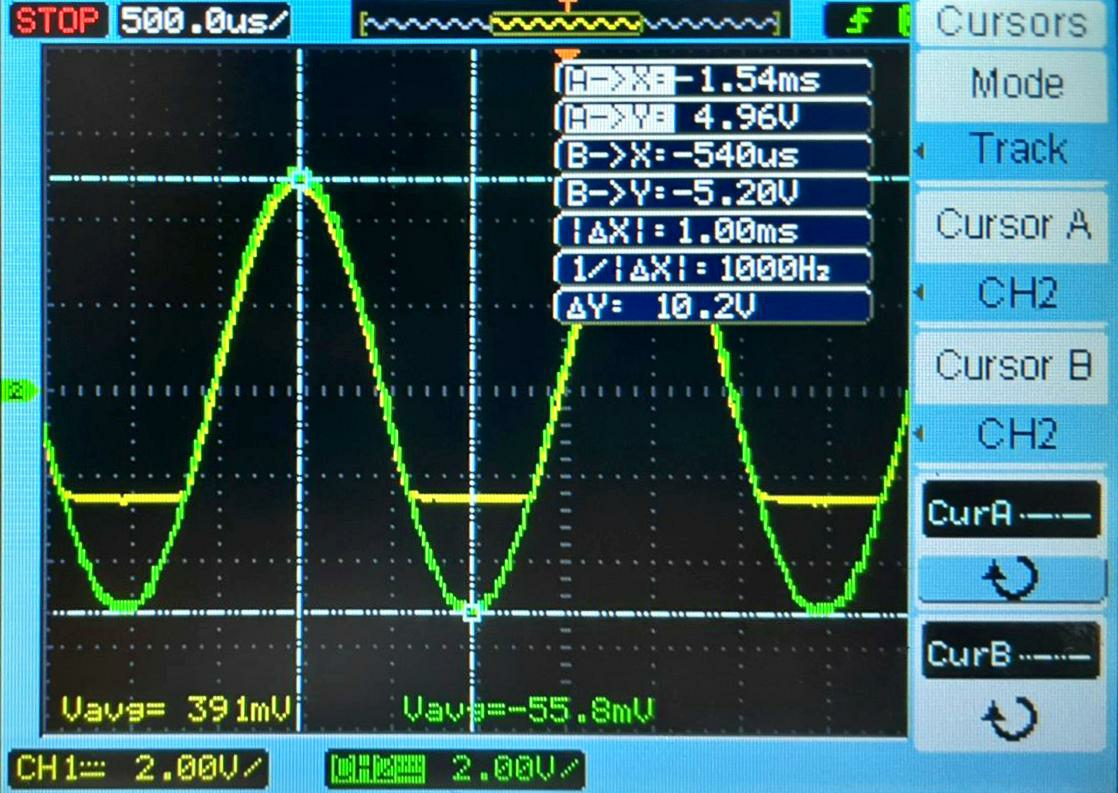
\includegraphics[width=0.9\columnwidth, height=110px]{1.jpeg}} \\ \vspace{5px}
D:+ \ S:+ \\

\columnbreak

\fcolorbox{black}{white}{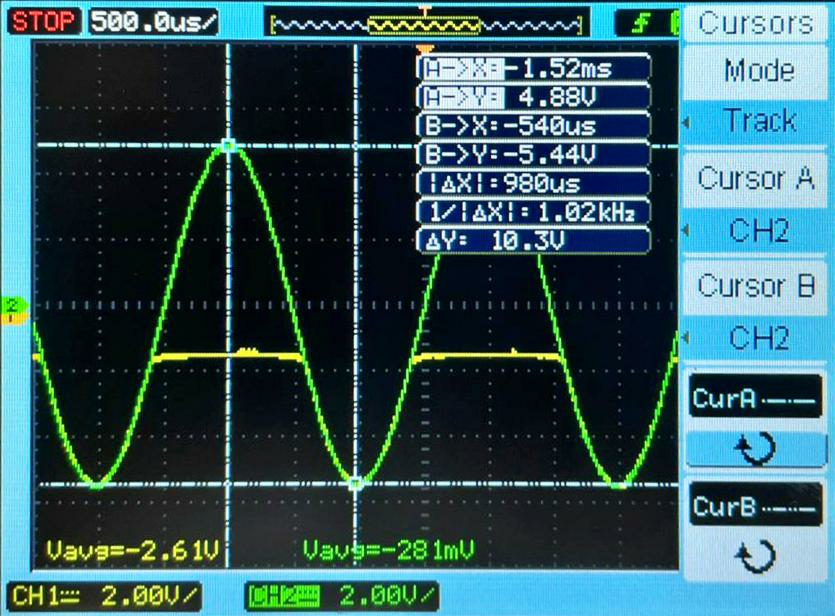
\includegraphics[width=0.9\columnwidth, height=110px]{2.jpeg}} \\ \vspace{5px}
D:- \ S:+
\end{center}
\end{multicols}
\begin{multicols}{2}
\begin{center}
\fcolorbox{black}{white}{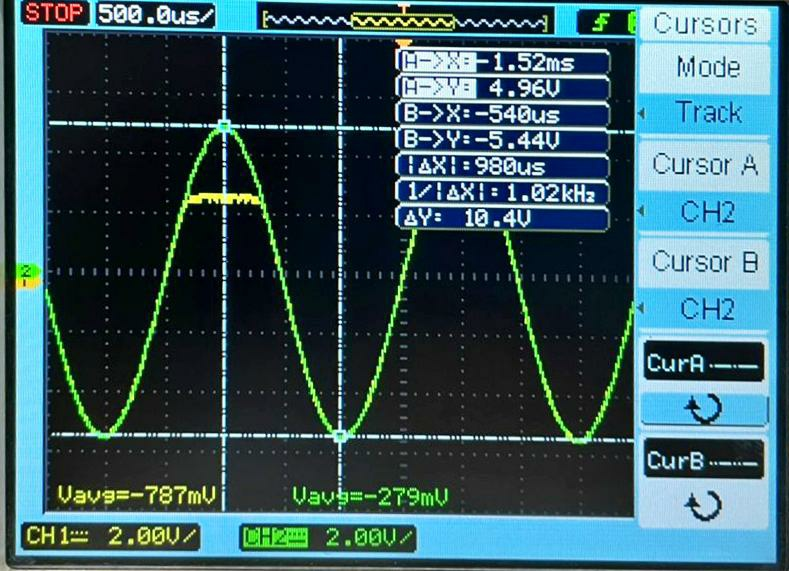
\includegraphics[width=0.9\columnwidth, height=110px]{3.jpeg}} \\ \vspace{5px}
D:- \ S:- \\

\columnbreak

\fcolorbox{black}{white}{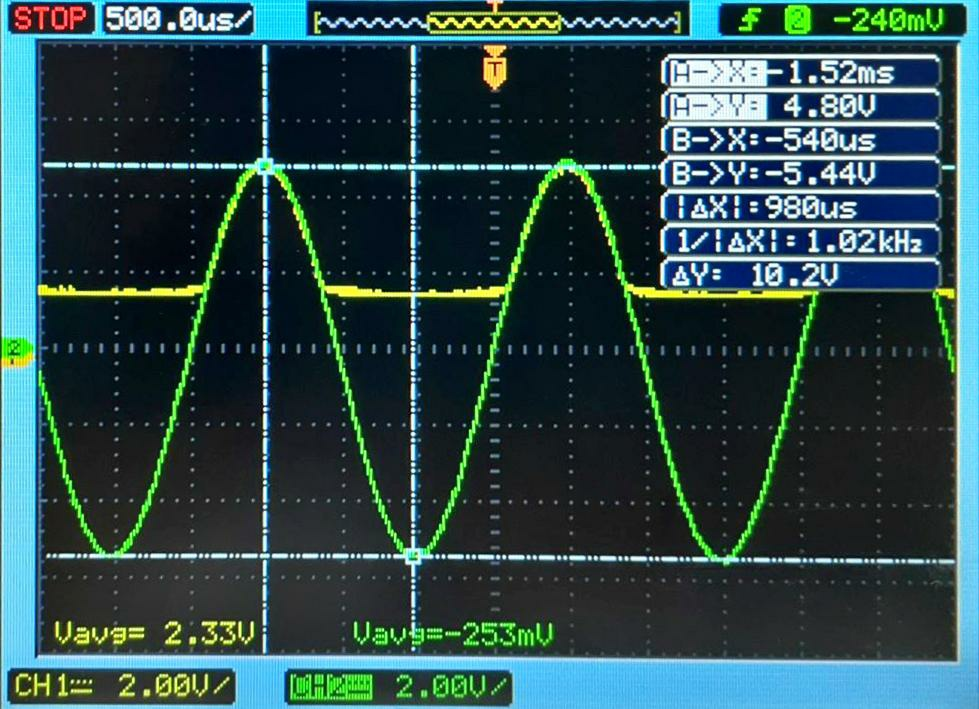
\includegraphics[width=0.9\columnwidth, height=110px]{4.jpeg}} \\ \vspace{5px}
D:+ \ S:- 
\end{center}
\end{multicols}

\subsection{Observation}
\vspace{5px}
\begin{center}
\begin{tabular}{| c | c | c | c | c |} 
 \hline
    \ & \ & \ & \ & \ \\
    Signal & $Input_{PP}$ & $Input_{avg}$ & $Output_{PP}$ & $Output_{avg}$ \\ [1em]
    \hline
    \ & \ & \ & \ & \ \\
    D:+ \ S:+  & 10.2V & -55.8mV & 7.36V & 391mV \\
    D:- \ S:+  & 10.3V & -281mV & 3.92V & -2.61V \\
    D:- \ S:-  & 10.4V & -279mV & 7.92V & -787mV \\
    D:+ \ S:-  & 10.2V & -253mV & 3.36V & 2.33V \\
    \ & \ & \ & \ & \ \\
 \hline
\end{tabular}
\end{center}

\subsection{Conclusion}
Hence we see the ouput waveforms for a Clipper circuit and observe the changes when we reverse the polarities of source or diode.



\newpage

\section{Diode Clamping}
\subsection{Aim}
To investigate the characteristic of diode clamping circuit.
\subsection{Apparatus}
\begin{enumerate}
\item Breadboard and Jumpers
\item Multimeter and Resistors
\item Capacitor ( Both Electrolytic and Non-Electrolytic)
\item Digital Storage Oscilloscope (DSO1052B)
\item Function Generator (0 – 3 MHz) and External Voltage
\end{enumerate}


\subsection{Theory}
\begin{wrapfigure}{R}{0.25\textwidth}
\fcolorbox{black}{white}{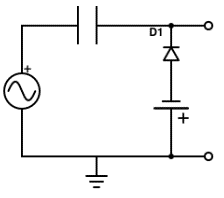
\includegraphics[width=0.25\textwidth]{Picture3.png}}
\end{wrapfigure}
A clamper is an electronic circuit that fixes either the positive or the negative peak excursions of a signal to a defined value by shifting its DC value. The clamper does not restrict the peak-to-peak excursion of the signal, it moves the whole signal up or down so as to place the peaks at the reference level. A diode clamp consists of a diode, and a capacitor which provides a DC offset from the stored charge. \\

\noindent
\textbf{Diode and Source Polarities are considered +ve as per the circuit on the right.}

\subsection{Breadboard Setup}
\vspace{5px}
\begin{center}
\fcolorbox{black}{white}{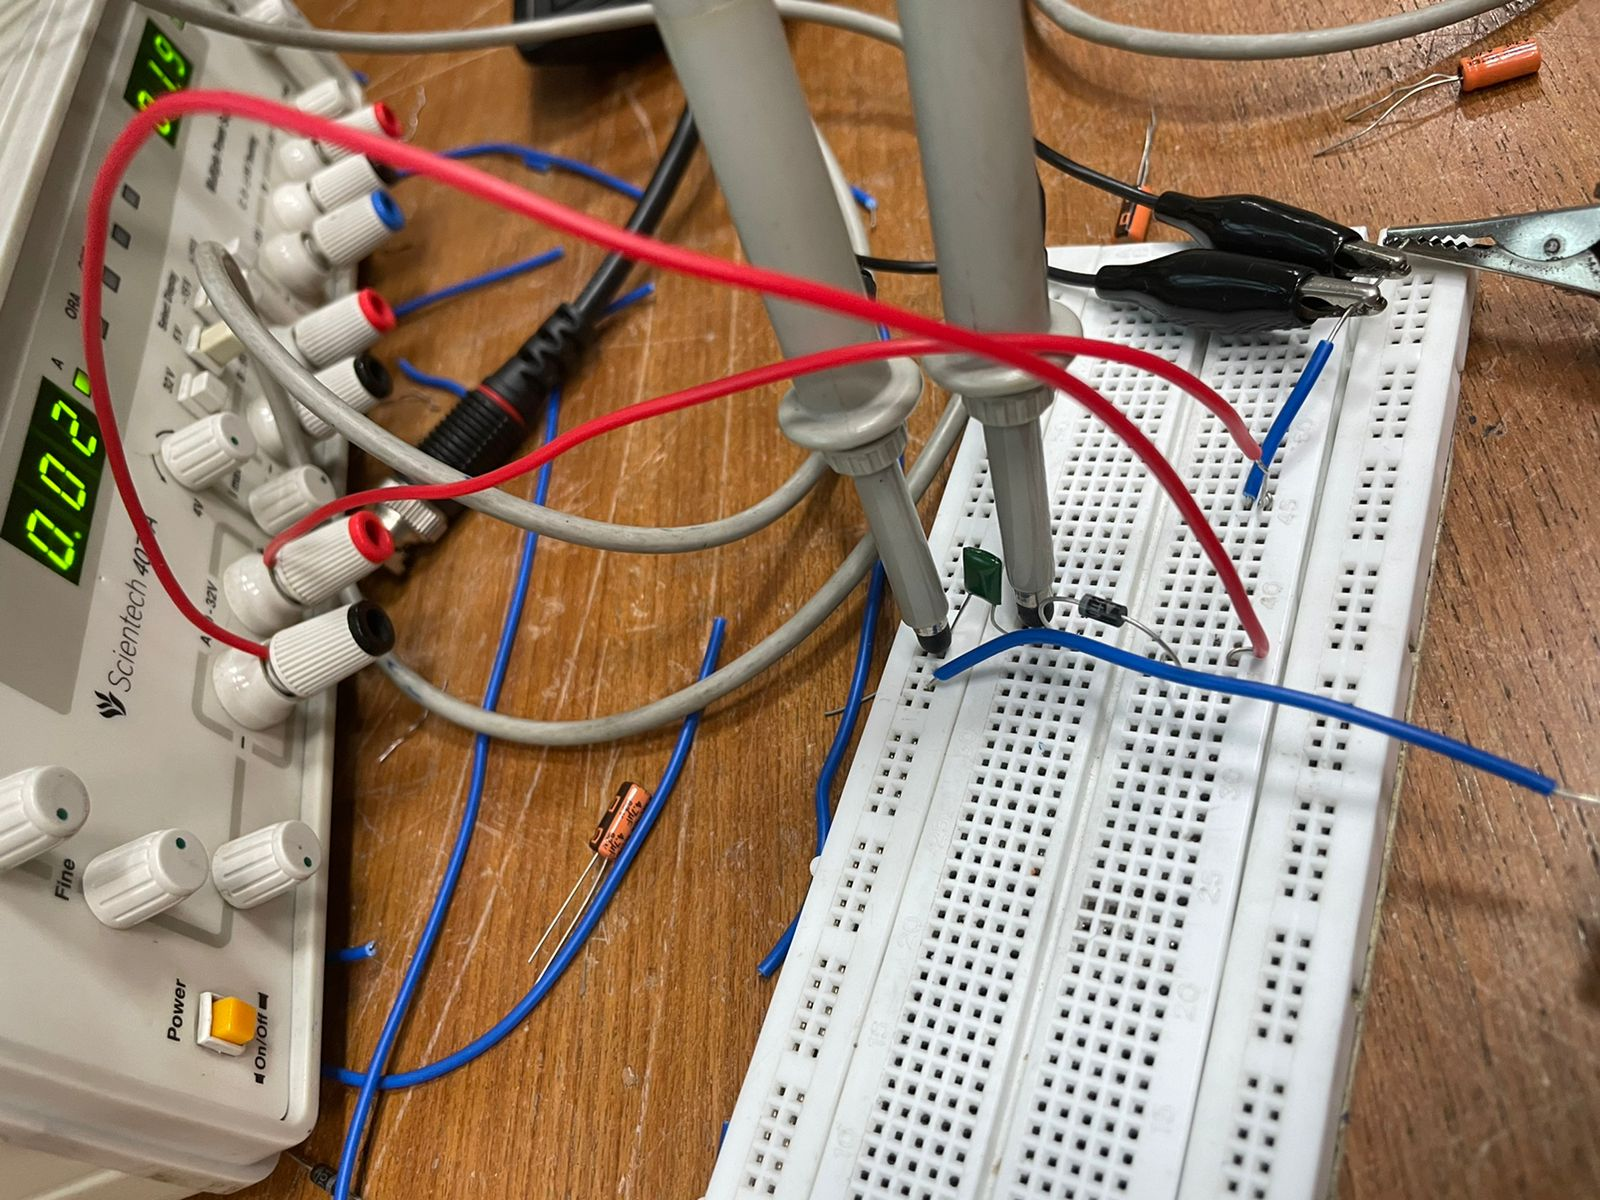
\includegraphics[width=0.9\columnwidth, height=130px]{WhatsApp Image 2022-04-27 at 4.39.53 PM.jpeg}} \\ \vspace{5px}
Circuit with $C=0.01 \mu F$ and V=2V\\
\end{center}

\subsection{Images of DSO}
\vspace{5px}
\begin{multicols}{2}
\begin{center}
\fcolorbox{black}{white}{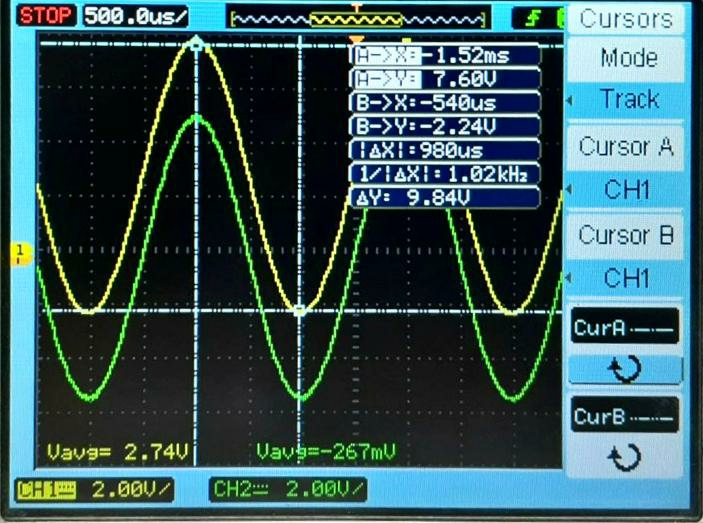
\includegraphics[width=0.9\columnwidth, height=110px]{44.jpeg}} \\ \vspace{5px}
D:+ \ S:+ \\

\columnbreak

\fcolorbox{black}{white}{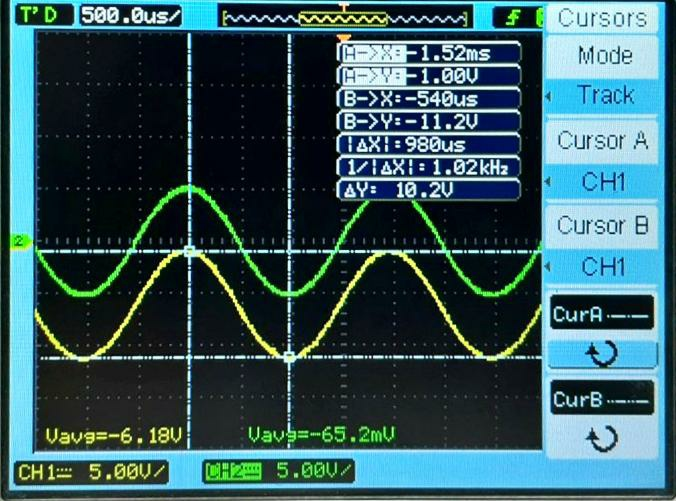
\includegraphics[width=0.9\columnwidth, height=110px]{33.jpeg}} \\ \vspace{5px}
D:- \ S:+
\end{center}
\end{multicols}
\begin{multicols}{2}
\begin{center}
\fcolorbox{black}{white}{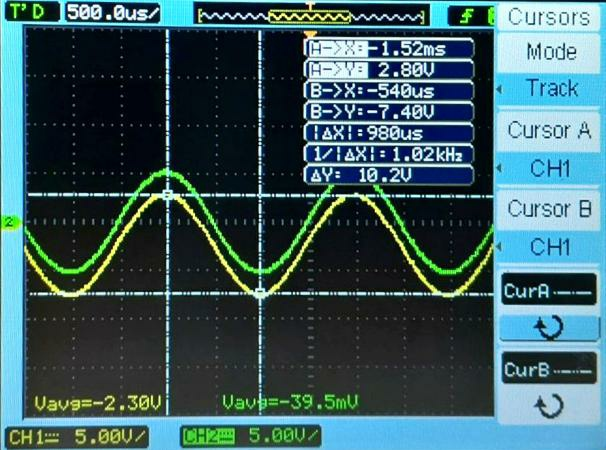
\includegraphics[width=0.9\columnwidth, height=110px]{22.jpeg}} \\ \vspace{5px}
D:- \ S:- \\

\columnbreak

\fcolorbox{black}{white}{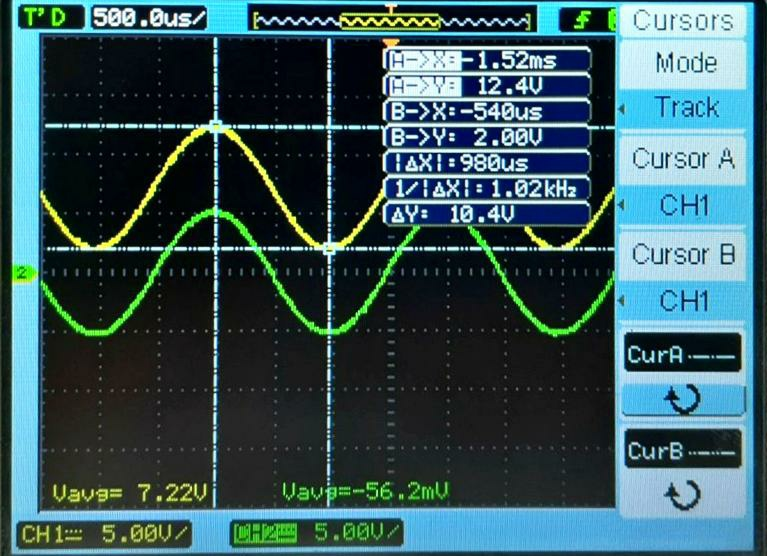
\includegraphics[width=0.9\columnwidth, height=110px]{11.jpeg}} \\ \vspace{5px}
D:+ \ S:- 
\end{center}
\end{multicols}

\subsection{Observation}
\vspace{5px}
\begin{center}
\begin{tabular}{| c | c | c | c | c |} 
 \hline
    \ & \ & \ & \ & \ \\
    Signal & $Input_{PP}$ & $Input_{avg}$ & $Output_{PP}$ & $Output_{avg}$ \\ [1em]
    \hline
    \ & \ & \ & \ & \ \\
    D:+ \ S:+  & 10.2V & -267mV & 9.84V & 2.74V \\
    D:- \ S:+  & 10.2V & -65.2mV & 10.2V & -6.18V \\
    D:- \ S:-  & 10.2V & -39.5mV & 10.2V & -2.30V \\
    D:+ \ S:-  & 10.2V & -56.2mV & 10.4V & 7.22V \\
    \ & \ & \ & \ & \ \\
 \hline
\end{tabular}
\end{center}

\subsection{Conclusion}
Hence we see the ouput waveforms for a Clamper circuit and observe the changes when we reverse the polarities of source or diode.


\newpage
\vspace{10px}
\section{Sources of Error}
\begin{itemize}
\item Scale of DSO not appropriate for measurements
\item Loose Connections
\item Resistance of wires not taken into account, and also giving rise to inconsistency due to increase in resistance due to heating
\item Change in the connections while circuit is closed.

\end{itemize}

\vspace{5px}

\section{Precautions}

\begin{itemize}
\item Make the connections neat and tight
\item Don’t leave the switch on for long continuous periods of time.
\item Wear proper shoes and use insulated tools
\end{itemize}

\vspace{5px}

\section{Concluding Remarks}
We investigated the use of a diode as a rectifier, in a clipping circuit, and in a clamping circuit in the experiment above. When only one diode is employed in a circuit, the result is a half wave rectifier, which permits only one part of the current cycle to pass through (positive or negative). The diode prevents the other half of the input wave from passing through, resulting in rectified voltage. \\

\noindent
A diode with a DC Source can be used in a clipping circuit to clip a portion of the input signal. The polarity of the diode decides which half is clipped, and the voltage of the DC Source sets the threshold voltage at which the wave signal is clipped above (or below). The outcomes were also as anticipated. \\

\noindent
In a clamping circuit, the voltage is moved by half the peak-to-peak value (ALso depends on external source) above or below its original mean position. The DSO screens show the same thing.  \\

\noindent
Thus, the diodes can effectively rectify, clip, or clamp AC signals.
\end{document}
